%%  THESIS TEMPLATE  %%%%%%%%%%%%%%%%%%%%%%%%%%%%%%%%%%%%%%%%%%%%%%%%%%%%%%%%%%%
%%
%%  Markus F. Weber (2016)
%%

\RequirePackage[l2tabu, orthodox]{nag}%  Reports deprecated or bad LaTeX code
\pdfminorversion=6%  version of the generated PDF, not really crucial

%% if you encounter ugly text on pages with figures:
%\pdfpageattr{/Group << /S /Transparency /I true /CS /DeviceRGB>>}


%%  FONT SIZE, PAGE LAYOUT, etc.  %%%%%%%%%%%%%%%%%%%%%%%%%%%%%%%%%%%%%%%%%%%%%%
%%
\documentclass[%  see KOMA-script documentation
  %
  % Some packages don't understand the british/american options.
  % Therefore, english is included as fallback option.
  % You may replace "british" by "american" both here and below in \selectlanguage
  %
  ngerman, english, british,% last option=default
  twoside,%
  12pt,%
  %DIV=10, BCOR=10mm,%  see below
  headinclude=true,%
  chapterprefix=false,% 
  appendixprefix=false,% 
  headings=normal,% see styling.tex for settings of headings
  numbers=noenddot,%
  bibliography=totoc,%  puts the bibliography into the table of contents
  final%  final / draft
]{scrbook}%  see KOMA-script documentation



%% A4 (PRINT, For Web: left=right=35mm might be more convenient)
%% > Based on the DIV=10/BCOR=10mm KOMA-script settings
%% > but with symmetric top/bottom margins
\usepackage[a4paper,% 
  %
  left=30mm,%
  right=40mm,%
  marginparwidth=27.5mm,%
  %
  top=43.5mm,%
  bottom=43.5mm%
]{geometry}



%%  PACKAGES, FONTS, STYLING, etc. %%%%%%%%%%%%%%%%%%%%%%%%%%%%%%%%%%%%%%%%%%%%%
%%
% Math packages
%%%%%%%%%%%%%%%%%%%%%%%%%%%%%%%%%%%%%%%
\usepackage{amsmath}
\usepackage{amsthm}
\usepackage{amssymb}
\usepackage{mathtools}

%  AMS packages, some basic math styling
% Basic packages
%%%%%%%%%%%%%%%%%%%%%%%%%%%%%%%%%%%%%%%
\usepackage[T1]{fontenc}%
\usepackage[utf8]{inputenc}%

\usepackage{babel}%
\usepackage[useregional]{datetime2}% custom formatted dates, used in author_info.tex
\usepackage{csquotes}%  Required by babel

\usepackage[draft=false]{scrlayer-scrpage}

\usepackage[full]{textcomp}% Fix warning with missing font shapes

\usepackage[font=small,format=plain,%  Customized figure captions 
   labelfont=bf,labelsep=space]{caption}%

\usepackage[draft=false]{microtype}%  Better spacing (ugly line breaks are corrected most easily in draft mode... deactivation of microtype in that mode might change the places at which lines are broken)

\usepackage{graphicx}%
\graphicspath{{./images/}}%  Graphics directory

\usepackage{tikz}% used for Feynman diagrams, see tikz.tex

\usepackage{ctable}%  tables with captions & footnotes

\usepackage{appendix}%  Appendices for individual chapters

\usepackage{setspace}%  sin­glespac­ing / onehalfspacing / doublespacing commands

\usepackage{enumitem}%  Some customization for enumerate

\usepackage{lastpage}%  Removes some warning

\usepackage{printlen}%  Print the width of the page, useful for figures
\uselengthunit{mm}

\usepackage{xpatch}%  For some custom patches

\usepackage{fnpct}%  automatically places footnote marks after punctuation marks as it should be

\usepackage{marginnote}%  Extension of the \marginpar command
\usepackage{ragged2e}%  hyphenation in margin notes... not too great
\renewcommand*{\raggedleftmarginnote}{\RaggedLeft}
\renewcommand*{\raggedrightmarginnote}{\RaggedRight}

\usepackage{xcolor}% colors defined in styling.tex

\usepackage{ellipsis}%  correct some whitespace issue for ellipses (doesn't work with XeLaTeX's mathspec?)

\usepackage{siunitx}% correct typesetting for dimensional numbers (e.g. \SI{1}{\micro\litre})

%  fontenc, inputenc, babel, ...

% ADD YOUR INFO TO THIS FILE (name, title of the thesis,...)
% General info
%%%%%%%%%%%%%%%%%%%%%%%%%%%%%%%%%%%%%%%

\newcommand*{\ThesisType}{PhD thesis}

\newcommand*{\mainTitle}{Thesis template}
\newcommand*{\subTitle}{The architectonic of pure design}
\newcommand*{\Title}{\mainTitle{}: \subTitle{}}
\newcommand*{\Keywords}{% keep the space before the % in a line break
   Critical philosophy, analytic judgement, synthetic judgement, %
   a priori, a posteriori, synthetic a priori%
}

\newcommand*{\Author}{Immanuel Kant Lipsum}
\newcommand*{\PlaceOfBirth}{K\"onigsberg}
\newcommand*{\EMail}{immanuel@kant.com}

\newcommand*{\University}{Hogwarts School of Aeronautics}
\newcommand*{\Department}{Faculty of Archery}

\newcommand*{\PlaceOfSubmission}{Rome}
\DTMsavedate{DateOfSubmission}{1123-09-08}
\DTMsavedate{DateOfOralExamination}{1123-10-27}

\newcommand*{\FirstReferee}{Prof.\ Dr.\ Baruch Spinoza}
\newcommand*{\SecondReferee}{Prof.\ Dr.\ Hilarius von Poitiers}%

%% If you use LuaLaTeX or XeLaTeX:
% > comment out \pdfminorversion in main.tex
% > comment out the other font files in main.tex
% > comment out inputenc & fontenc in basic_packages.tex
% > comment out \pdfpageattr in pdfs.tex
% > remove pdftex in hyperref_metadata.tex

% in case you own these fonts... legally


%% Serif (LuaLaTex)
%%%%%%%%%%%%%%%%%%%%%%%%%%%%%%%%%%%%%%%
%\usepackage[adobe-garamond,expert]{mathdesign}% math for Garamond
%
%\usepackage[no-math]{fontspec}
%
%\setmainfont[%
%	Ligatures={TeX,Common}
%]{Adobe Garamond Pro}% EB Garamond, Adobe Garamond Pro, Garamond Premier Pro


%% Serif (XeLaTeX)
%%%%%%%%%%%%%%%%%%%%%%%%%%%%%%%%%%%%%%%
\usepackage{mathspec}

\setmainfont[%
	Ligatures={TeX,Common}
]{Adobe Garamond Pro}% EB Garamond, Adobe Garamond Pro, Garamond Premier Pro

\setmathsfont(Digits,Latin,Greek)[%
	Numbers={Proportional}%
]{EB Garamond}

\setmathrm{EB Garamond}

\AtBeginEnvironment{tabular}{%
	\addfontfeature{RawFeature=+tnum}
}

\newfontfamily{\smallcaps}[%
	RawFeature={+c2sc,+scmp}%
]{EB Garamond}


%% Sans serif 
%%%%%%%%%%%%%%%%%%%%%%%%%%%%%%%%%%%%%%%
\setsansfont[%
	Ligatures=TeX%,%
	%Scale=MatchLowercase%
]{Linux Biolinum O}%  Lato Regular  


%% Typewriter 
%%%%%%%%%%%%%%%%%%%%%%%%%%%%%%%%%%%%%%%
\setmonofont[%
	Ligatures=TeX%,%
	%Scale=MatchLowercase%
]{Inconsolata}%  Linux Biolinum O, Source Code Pro% If you prefer LuaLaTeX or XeLaTeX
%% Fonts with math support: http://www.tug.dk/FontCatalogue/mathfonts.html



% Installation of garamondx and Baskervaldx (http://tug.org/fonts/getnonfreefonts/):
%  run the following commands in garamondx folder:
%  > sudo texlua install-getnonfreefonts (no responsibility for damages ;) )
%  > getnonfreefonts garamondx
%  > getnonfreefonts Classico
%  > getnonfreefonts Baskervaldx



%  Times
%%%%%%%%%%%%%%%%%%%%%%%%%%%%%%%%%%%%%%%
% comes with sans serif and typewriter font (comment out those files in main.tex)
%\usepackage{newtxtext}
%\usepackage[bigdelims]{newtxmath}


%  URW Garamond No.8 (optimized)
%%%%%%%%%%%%%%%%%%%%%%%%%%%%%%%%%%%%%%%
%  There's some warnings on missing fonts for garamondx... 
%  but I didn't see any problems in the output.
\usepackage{garamondx}%  [osf] 
\usepackage[garamondx,bigdelims]{newtxmath}%  mods: cmintegrals

% Modify math fonts for \mathbb, \mathcal, etc.
%%%%%%%%%%%%%%%%%%%%%%%%%%%%%%%%%%%%%%%
% should be loaded after other math font packages as far as I know
\usepackage[cal=cm]{mathalfa}%  see package doc for options


%%  EB Garamond
%%%%%%%%%%%%%%%%%%%%%%%%%%%%%%%%%%%%%%%% 
%% > lacks some math symbols (e.g. \partial)
%
%\usepackage{ebgaramond}%  
%\usepackage[bigdelims]{newtxmath}%
%\usepackage{ebgaramond-maths}%  ugly spacing in fractions
%%  EB Garamond doesn't have a bold version.
%%  Could possibly replace bold by swash (textbf -> textsw)
%%  OR: Fake bold with the following two lines (needs ``getnofreefonts garamond'' for bold URW Garamond)
%\newcommand{\fakebf}{\fontfamily{mdugm}\fontseries{b}\selectfont}% These two lines fake bold Garamond.
%\DeclareTextFontCommand{\textbf}{\fakebf}%  But it's not really EB Garamond.


%  Baskerville (optimized)
%%%%%%%%%%%%%%%%%%%%%%%%%%%%%%%%%%%%%%%
%\usepackage{Baskervaldx}%  mods: osf, ...
%\usepackage[baskervaldx,bigdelims]{newtxmath}


%  Bitstream Charter (optimized)
%%%%%%%%%%%%%%%%%%%%%%%%%%%%%%%%%%%%%%%
%\usepackage[scaled=.98,sups]{XCharter}%  mods: osf, ...
%\usepackage[charter,bigdelims,scaled=1.07]{newtxmath}%  mods: vvarbb, scaled=1.04


%  Linux Libertine
%%%%%%%%%%%%%%%%%%%%%%%%%%%%%%%%%%%%%%%
%\usepackage{libertineRoman}
%\usepackage[libertine,bigdelims]{newtxmath}


%  Latin Modern (corresponding "unicode-math" package only available in XeLaTeX/LuaLaTeX)
%%%%%%%%%%%%%%%%%%%%%%%%%%%%%%%%%%%%%%%
%\usepackage{lmodern}


%  Minion Pro
%%%%%%%%%%%%%%%%%%%%%%%%%%%%%%%%%%%%%%%
%\usepackage{MinionPro}%  Provides both serif text & math (comment the stuff below)
%\usepackage{MnSymbol}


%  Palatino
%%%%%%%%%%%%%%%%%%%%%%%%%%%%%%%%%%%%%%%
%\usepackage{mathpazo}%  Palatino (text and math... don't know why
%\usepackage{eulervm}%  Euler math is always suggested for it)


%  Utopia
%%%%%%%%%%%%%%%%%%%%%%%%%%%%%%%%%%%%%%%
%\usepackage[scaled=.98]{erewhon}%  mods: osf, ...
%\usepackage[utopia,vvarbb,bigdelims]{newtxmath}



%  Sans-serif fonts: http://www.tug.dk/FontCatalogue/sansseriffonts.html

%  Linux Biolinum
%%%%%%%%%%%%%%%%%%%%%%%%%%%%%%%%%%%%%%%
%\usepackage{biolinum}%  [osf]

%  Optima clone "Classico" (sudo getnonfreefonts Classico)
%%%%%%%%%%%%%%%%%%%%%%%%%%%%%%%%%%%%%%%
\usepackage[scaled=0.95]{classico}% 


%  Source Sans Pro
%%%%%%%%%%%%%%%%%%%%%%%%%%%%%%%%%%%%%%%
%\usepackage{sourcesanspro}


%  Cabin
%%%%%%%%%%%%%%%%%%%%%%%%%%%%%%%%%%%%%%%
%\usepackage[type1]{cabin}%  mods: scaled=.95


%  Open Sans
%%%%%%%%%%%%%%%%%%%%%%%%%%%%%%%%%%%%%%%
%\usepackage{opensans}% mods: osfigures, scale=0.95


%  Classico
%%%%%%%%%%%%%%%%%%%%%%%%%%%%%%%%%%%%%%%
%\usepackage{classico}%  getnofreefonts classico


% PS: I don't really use the typewriter font, see hyperref_metadata.tex


% Typewriter: Inconsolata
%%%%%%%%%%%%%%%%%%%%%%%%%%%%%%%%%%%%%%%
\usepackage[varqu,varl]{zi4}%  Inconsolata  (mods: scaled=1.04)


% Typewriter: Libertine Mono
%%%%%%%%%%%%%%%%%%%%%%%%%%%%%%%%%%%%%%%
%\usepackage{libertineMono}%


% Inclusion of PDFs (publications)
%%%%%%%%%%%%%%%%%%%%%%%%%%%%%%%%%%%%%%%

\usepackage{pdfpages}		

% Counters for references to the page numbers of the PDFs
\newcounter{includepdfpage}
\newcounter{currentpagecounter}
\newcommand{\addlabelstoallincludedpages}[1]{%
  \refstepcounter{includepdfpage}%
  \stepcounter{currentpagecounter}%
  \label{#1.\thecurrentpagecounter}%
}
\newcommand{\modifiedincludepdf}[3]{%
  \setcounter{currentpagecounter}{0}%
  \includepdf[#1,pagecommand={\addlabelstoallincludedpages{#2}\thispagestyle{empty}}]{#3}%
}

%  inclusion of full-page PDFs (for publications)
% Epigraphs
%%%%%%%%%%%%%%%%%%%%%%%%%%%%%%%%%%%%%%%

\usepackage{epigraph}
\renewcommand{\textflush}{flushright}
\setlength\epigraphwidth{\textwidth}
\setlength\epigraphrule{0pt}

% Remove page number from epigraphstyle 
% Otherwise there's a centered page number on first page of chapters
\makeatletter%
   \xpatchcmd\epigraphhead%
  {\let\@evenfoot}%
  {\let\@oddfoot\@empty\let\@evenfoot}%
  {}{}%
\makeatother

% Bibliography style
%%%%%%%%%%%%%%%%%%%%%%%%%%%%%%%%%%%%%%%

% The bibliography really isn't optimal...
% Someone who knows how to modify .bbx files should have a look at custom-numeric-comp.bbx.
% I found that file on the web but did some modifications to it.
% I tried to add an Oxford comma to the bibliography but didn't succeed.
% (there's a dictionary for Oxford spelling in ./etc/ , needed that for an IOP article)
 
% Some citations to different sources are included in ch.2 (article, book, inbook, proceedings, etc.).
% A good alternative to biber is to use bibtex with the unsrturl.bst stylefile (back-refs don't work then).

\usepackage[%
   backend=biber,%
   bibencoding=utf8,%
   style=custom-numeric-comp,%  nice compact number style
   giveninits=true,%  abbreviate author names
   hyperref=true,%  have links, requires hyperref
   doi=true,%  have doi links
   url=false,%  no urls
   isbn=false,%  no isbn numbers
   arxiv=false,%  no arXiv
   backref=true,%  have back references to citation location
   sorting=none,%  have citations appear in the order they are cited
   abbreviate=true,%  use abbreviations, e.g. for months
   defernumbers=true,%  required by resetnumbers
   maxbibnames =10%  abbreviate et.al. for four authors and more
]{biblatex}

\renewbibmacro{in:}{}%  no "In:" after title
\DeclareFieldFormat[article]{pages}{#1}%  no p./pp. for articles (b./c. the single numbers in e.g. PRL are no page numbers?)
\DeclareFieldFormat[article]{volume}{\textbf{#1}}%  bold volume number for articles
\DeclareFieldFormat[inbook,book,thesis]{title}{\textit{#1}}%  italic title
\DeclareFieldFormat[article,unpublished,inproceedings,incollection,online]{title}{#1}%      normal title
  
% Makes the "et al" italicized bibliography
\xpatchbibmacro{name:andothers}{%
   \bibstring{andothers}%
   }{%
   \bibstring[\emph]{andothers}%
   }{}{}

%%  Custom colors
%%%%%%%%%%%%%%%%%%%%%%%%%%%%%%%%%%%%%%%
\definecolor{myGreen}{rgb}{0.072 0.42 0.03}
\definecolor{myLightBlue}{rgb}{0. 0.35 0.68}
\definecolor{myBlue}{rgb}{0.28 0.36 0.48}
\definecolor{myRed}{rgb}{0.65 0.04 0.07}
\definecolor{myPurple}{rgb}{0.52 0. 0.53}


%%  Style of margin notes
%%%%%%%%%%%%%%%%%%%%%%%%%%%%%%%%%%%%%%%
\renewcommand*{\marginfont}{\small}


%%  Style of footnotes
%%%%%%%%%%%%%%%%%%%%%%%%%%%%%%%%%%%%%%%
%  use indent OR line
%  for a paragraph style indent choose 2.5em (1+1.5em)
\deffootnote{1em}{0em}{\thefootnotemark\hspace*{.5em}}%


%%  Font size on cover page
%%%%%%%%%%%%%%%%%%%%%%%%%%%%%%%%%%%%%%%
\makeatletter%
	\renewcommand\Huge{\@setfontsize\Huge{29}{34.8}}%
\makeatother


%%  Kill widows and orphans
%%%%%%%%%%%%%%%%%%%%%%%%%%%%%%%%%%%%%%%
\usepackage[all,defaultlines=2]{nowidow}%  at least 2 lines at bottom and top of pages


%%  Line spread
%%%%%%%%%%%%%%%%%%%%%%%%%%%%%%%%%%%%%%%
%\linespread{1.04}


%%  Style of chapter & section headlines
%%%%%%%%%%%%%%%%%%%%%%%%%%%%%%%%%%%%%%%

%% quotchap
%\usepackage[palatino]{quotchap}
%\renewcommand*{\chapterheadstartvskip}{\vspace*{-1.5\baselineskip}}
%\renewcommand*{\chapterheadendvskip}{\vspace{1.3\baselineskip}}
%\definecolor{chaptergrey}{rgb}{0.6 0.6 0.6} % colour of chapter number


%% KOMA script
%% all headings
%\setkomafont{disposition}{\color{myBlue}\sffamily\bfseries}%   changes all headings

%% fonts of headings
%\setkomafont{chapter}{\fontsize{18}{21.6}\selectfont}
%\setkomafont{section}{\fontsize{14}{16.8}\selectfont}
%\setkomafont{subsection}{\fontsize{13}{15.6}\selectfont}
%\setkomafont{subsubsection}{\fontsize{12.5}{15}\selectfont}
%\setkomafont{paragraph}{\fontsize{12}{14.4}\selectfont}
%\setkomafont{subparagraph}{\fontsize{12}{14.4}\selectfont}

%% positions of headings
%\RedeclareSectionCommand[beforeskip=-1.6\baselineskip, afterskip=1.4\baselineskip]{chapter}% default: -3 / 1.4
%\RedeclareSectionCommand[beforeskip=-\baselineskip, afterskip=.5\baselineskip]{section}
%\RedeclareSectionCommand[beforeskip=-.5\baselineskip, afterskip=0.25\baselineskip]{subsection}
%\RedeclareSectionCommand[beforeskip=-.25\baselineskip,afterskip=1sp]{subsubsection}
%\RedeclareSectionCommands[beforeskip=-.25\baselineskip,afterskip=1sp]{paragraph}%  introduces a line break after paragraph headings
  
  

%%  Paragraph indentation & spacing
%%%%%%%%%%%%%%%%%%%%%%%%%%%%%%%%%%%%%%%
% It's typically considered bad style to use both indent and spacing (check any book you have)
% Note that additional \parskip also affects the space around headings. 
% Those spaces can be changed with the options above.
\setlength{\parindent}{1.5em}%  Indent new paragraph
\setlength{\parskip}{0\baselineskip}%  Space between paragraphs
%%%%%%%%%%%%%%%%%%%%%%%%%%%%%%%%%%%%%%%





%%  Table of contents & Numbering
%%%%%%%%%%%%%%%%%%%%%%%%%%%%%%%%%%%%%%%
% I decided against the numbering of sections, figures, and equations by chapters:

% depth (3=subsubsection)
\setcounter{secnumdepth}{3}%
\setcounter{tocdepth}{3}

%% Nice style:
%\usepackage[tocgraduated]{tocstyle}
%\usetocstyle{nopagecolumn}


%% I used the following style (the chapter number before the subappendix is hidden in project_1.tex)
%% numbers
%\renewcommand{\theequation}{\arabic{equation}}%  running equation number in chapters
%\renewcommand{\thefigure}{\arabic{figure}}%  running figure number in chapters
%\renewcommand{\thetable}{\arabic{table}}%  running table number in chapters

%% numbers (comment out for standard appearance)
\renewcommand\thechapter{\Roman{chapter}}
\renewcommand\thesection{\thechapter.\arabic{section}}
\renewcommand\thesubsection{\thesection.\arabic{subsection}}
\renewcommand\thesubsubsection{\thesubsection \alph{subsubsection}}

%% spacing (comment out for standard appearance)
%\makeatletter
%  \renewcommand*\l@section{\bprot@dottedtocline{1}{1.5em}{1.25em}}
%  \renewcommand*\l@subsection{\bprot@dottedtocline{2}{2.75em}{1.99em}}
%  \renewcommand*\l@subsubsection{\bprot@dottedtocline{3}{4.74em}{2.65em}}
%  \renewcommand*\@pnumwidth{2em}
%\makeatother
%%%%%%%%%%%%%%%%%%%%%%%%%%%%%%%%%%%%%%%



%% IF YOU HAVE TROUBLE WITH FLOATS UNCOMMENT THE FOLLOWING LINES
%
%% I didn't see any use for them in my documents.
%% maybe they are already integrated in the KOMA script?

%% Alter some LaTeX defaults for better treatment of figures:
%% See p.105 of "TeX Unbound" for suggested values.
%% See pp. 199-200 of Lamport's "LaTeX" book for details.
%
%%  General parameters, for ALL pages:
%\renewcommand{\topfraction}{0.9}%  max fraction of floats at top
%\renewcommand{\bottomfraction}{0.8}%  max fraction of floats at bottom
%
%%  Parameters for TEXT pages (not float pages):
%\setcounter{topnumber}{1}
%\setcounter{bottomnumber}{2}
%\setcounter{totalnumber}{4}%  2 may work better
%\setcounter{dbltopnumber}{2}%  for 2-column pages
%\renewcommand{\dbltopfraction}{0.9}%  fit big float above 2-col. text
%\renewcommand{\textfraction}{0.07}%  allow minimal text w. figs
%%  Parameters for FLOAT pages (not text pages):
%\renewcommand{\floatpagefraction}{0.7}%  require fuller float pages
%%  N.B.: floatpagefraction MUST be less than topfraction !!
%\renewcommand{\dblfloatpagefraction}{0.7}%  require fuller float pages
%%  remember to use [htp] or [htpb] for placement
%%%%%%%%%%%%%%%%%%%%%%%%%%%%%%%%%%%%%%%%

%or
%\renewcommand{\topfraction}{0.85}
%\renewcommand{\textfraction}{0.1}
%\renewcommand{\floatpagefraction}{0.85}

%  indentation, TOC, header, footer, ...
% TikZ for Feynman diagrams
%%%%%%%%%%%%%%%%%%%%%%%%%%%%%%%%%%%%%%%
\usetikzlibrary{positioning}
\usetikzlibrary{arrows.meta}
\usetikzlibrary{decorations.markings}
\usetikzlibrary{calc}
   
\tikzset{
   linePlain/.style={draw=black, thick},
   lineWithArrow/.style={draw=black, thick, postaction={decorate},decoration={markings,mark=at position .6 with {\arrow[scale=1.75]{stealth}}}},
   lineWithArrowInline/.style={draw=black, semithick, postaction={decorate},decoration={markings,mark=at position .7 with {\arrow[scale=1.75]{stealth}}}},
   vertex/.style={draw, shape=circle, fill=black, minimum size=1.1mm, inner sep=0mm, outer sep=0mm},
}
\newcommand{\upperloop}[3][]{%
   \draw[#1] let \p1 = ($(#2)-(#3)$) in (#2) arc (0:180:({0.5*veclen(\x1,\y1)});)
} 
\newcommand{\lowerloop}[3][]{%
   \draw[#1] let \p1 = ($(#2)-(#3)$) in (#2) arc (360:180:({0.5*veclen(\x1,\y1)});)
} 
%%%%%%%%%%%%%%%%%%%%%%%%%%%%%%%%%%%%%%%

%  for Feynman diagrams
% Roman numerals
%%%%%%%%%%%%%%%%%%%%%%%%%%%%%%%%%%%%%%%
\makeatletter%
	\newcommand{\rmnum}[1]{\romannumeral #1}%
	\newcommand{\Rmnum}[1]{\expandafter\@slowromancap\romannumeral #1@}%
\makeatother


% Copyright symbol
%%%%%%%%%%%%%%%%%%%%%%%%%%%%%%%%%%%%%%%
%\newcommand*{\myCopyrightLarge}{\textsf{\large\textcopyright}}
%\newcommand*{\myCopyrightNormal}{\textsf{\large\textcopyright}}
\newcommand*{\myCopyrightLarge}{\textsf{\raisebox{-0.79ex}{\fontsize{20pt}{24}\selectfont\textcopyright}}}
\newcommand*{\myCopyrightNormal}{\textsf{\raisebox{-0.81ex}{\fontsize{17.5pt}{20.4}\selectfont\textcopyright}}}




% Miscellaneous
%%%%%%%%%%%%%%%%%%%%%%%%%%%%%%%%%%%%%%%
\newenvironment{customCenter}[1][\topsep]
  {\setlength{\topsep}{#1}\par\kern\topsep\centering}% \begin{customCenter}[<len>]
  {\par\kern\topsep}% \end{customCenter}
% 
% Some useful definitions
%%%%%%%%%%%%%%%%%%%%%%%%%%%%%%%%%%%%%%%
% (some are only included because I needed them for an IOP review)

% Theorem environment (amsthm package)
\newtheoremstyle{customTheorem}% name
	{1ex}% Space above
	{1ex}% Space below
	{}% Body font
	{0pt}% Indent amount
	{\bfseries}% Theorem head font
	{}% Punctuation after theorem head
	{5pt plus 1pt minus 1pt}% Space after theorem head
	{}% Theorem head spec (can be left empty, meaning ‘normal’) 
\theoremstyle{customTheorem}
\newtheorem{theorem}{Theorem}

% Left/right parentheses (mathtools package)
\DeclarePairedDelimiter\paren{\lparen}{\rparen}

% Text in Equations
\newcommand*{\mathtext}[1]{\mathrm{#1}}
\newcommand*{\mathtextit}[1]{\mathit{#1}}

% Exponential and imaginary unit (were required to be upright for IOP)
\newcommand*{\ee}{\mathrm{e}}
\newcommand*{\ii}{\mathrm{i}} 

% Bold italic vector
\newcommand\hmmax{0}%  Patch for bm. With garamondx, the bold italic vector looks better,
\newcommand\bmmax{0}%  it's not great...but ok. Don't know why.
\usepackage{bm}%
\newcommand*{\vect}[1]{\bm{#1}}  

% Unit matrix
\usepackage{dsfont}

% Miscellaneous
\newcommand*{\bigO}{\mathord{\mathrm{O}}}
\newcommand*{\transpose}{\intercal}
\newcommand*{\laplaceOp}{\Delta}
\newcommand*{\discreteLaplaceOp}{\underline{\Delta}}
\newcommand*{\unitMatrix}{\mathds{1}}
\newcommand*{\hermite}{\mathit{He}}
\newcommand*{\legendreTransform}{\mathcal{L}}
\newcommand*{\fourierTransform}{\mathcal{F}}
\newcommand*{\complexPath}{\mathcal{C}}
\newcommand*{\binomCoeff}[2]{\binom{#1}{#2}}
\DeclareMathOperator{\Res}{Res}

% Sets
\newcommand*{\naturals}{\mathbb{N}}
\newcommand*{\integers}{\mathbb{Z}}
\newcommand*{\rationals}{\mathbb{Q}}
\newcommand*{\reals}{\mathbb{R}}
\newcommand*{\complex}{\mathbb{C}}
\newcommand*{\quaternions}{\mathbb{H}}
\newcommand*{\octonions}{\mathbb{O}}
\newcommand*{\lattice}{\mathbb{L}}

% Mathematical functions
\newcommand*{\arcosh}[1]{\mathtext{arcosh}\,#1}
 
% Differentials and integral signs
\newcommand*{\diff}{\mathop{}\!\mathrm{d}}
\usepackage{esint}%  Some more integral signs

% Fock space operations
\newcommand*{\numberOperator}{\mathsf{n}}
\newcommand*{\cre}{\mathsf{c}}
\newcommand*{\ann}{\mathsf{a}}

% Bra-ket notation (little bit optimized for garamondx... not optimal)
\newcommand*{\LLangle}{\langle\kern-2\nulldelimiterspace\langle\kern0.25\nulldelimiterspace}
\newcommand*{\bigLangle}{\big\langle}
\newcommand*{\bigLLangle}{\bigLangle\kern-2.25\nulldelimiterspace\bigLangle}
\newcommand*{\BigLangle}{\Big\langle}
\newcommand*{\BigLLangle}{\BigLangle\kern-2.35\nulldelimiterspace\BigLangle}

\newcommand*{\RRangle}{\rangle\kern-2\nulldelimiterspace\rangle}
\newcommand*{\bigRangle}{\big\rangle}
\newcommand*{\bigRRangle}{\bigRangle\kern-2.25\nulldelimiterspace\bigRangle}
\newcommand*{\BigRangle}{\Big\rangle}
\newcommand*{\BigRRangle}{\BigRangle\kern-2.35\nulldelimiterspace\BigRangle}

\newcommand*{\langleKern}{\langle\kern0.25\nulldelimiterspace}
\newcommand*{\vertLeft}{|\kern0.5\nulldelimiterspace}
\newcommand*{\vertRight}{\kern0.25\nulldelimiterspace|}
\newcommand*{\vertCenter}{\kern0.25\nulldelimiterspace|\kern0.5\nulldelimiterspace}

\newcommand*{\braA}[1]{{\langleKern #1 \vertRight}}
\newcommand*{\ketA}[1]{{\vertLeft #1 \rangle}}
\newcommand*{\braketA}[2]{\langleKern #1 \vertCenter #2 \rangle}

\newcommand*{\braB}[1]{\LLangle #1 \vertRight}
\newcommand*{\ketB}[1]{\vertLeft #1 \RRangle}
\newcommand*{\braketB}[2]{\LLangle #1 \vertCenter #2 \RRangle}

\newcommand*{\braketBA}[2]{\LLangle #1 \vertCenter #2 \rangle}
\newcommand*{\braketAB}[2]{\langleKern #1 \vertCenter #2 \RRangle}
%  some math shortcuts
% Temporary stuff (delete in final Doc?)
%%%%%%%%%%%%%%%%%%%%%%%%%%%%%%%%%%%%%%%

% Various packages
\usepackage{verbatim}%  Multiline comments
\usepackage[normalem]{ulem}%  Crossing stuff out with \sout{}
\usepackage{kantlipsum}%  Random text generator
%\usepackage[pagewise]{lineno}%  Line numbers

% Author notes - can be hidden by switching the %s
\newcommand{\mnote}[1]{{\color{myPurple}[M: #1]}}%  my own notes (M = Markus)
%\newcommand{\mnote}[1]{}

% Multiline comments - can be hidden by switching the %s
\newenvironment{commentDetails}{\ \newline\color{purple} Comment (additional details):}{\ignorespacesafterend\ \newline}
%\newcommand{\commentDetails}{\comment}

\usepackage[noframe]{showframe}%  for comments in the draft (remove in final version)
% Hyperrefs and PDF metadata
%%%%%%%%%%%%%%%%%%%%%%%%%%%%%%%%%%%%%%%

\PassOptionsToPackage{hyphens}{url}%  Correct line breaks of URLs
\urlstyle{rm}%  tt=typewriter; I did not like the typewriter DOIs in the bibliography

\usepackage{hyperxmp}

\usepackage[%
  pdftex,%
  pdfpagemode = {UseNone},%  required by the LMU library
  bookmarks,%
  plainpages=false,%
  pdfpagelabels,%
  %
  pdftitle={\Title{}},%  required by the LMU library
  pdfauthor={\Author{}},%  required by the LMU library
  pdfdate={\pdfcreationdate},%
  pdfcopyright={Copyright (c) \the\year, \Author{}},%
  pdfsubject={\ThesisType{}},%
  pdfkeywords={\Keywords{}},%
  pdfcontactemail={\EMail{}},%
  pdflang={en}%
]{hyperref}
  
%% FOR THE PRINT VERSION
%\hypersetup{%
%	hidelinks%  
%}

%% FOR THE ONLINE VERSION
\hypersetup{%
  colorlinks = true,%
  linkcolor = myLightBlue,%  myGreen
  urlcolor  = myGreen,%
  citecolor = myLightBlue,%  anchorcolor / menucolor... don't know what they are for
  linktocpage% makes the page number hyperlinks (looks better)
}

\usepackage{url}% There's some reason it's down here. 

\usepackage[noabbrev]{cleveref}% for internal links to sections, chapters, figures,...
\crefname{equation}{}{}
\newcommand{\crefrangeconjunction}{--}


%  Hyperrefs, metadata, load after general_info
\usepackage[acronym,toc,nopostdot,nonumberlist]{glossaries}% nonumberlist -> no backrefs

\glsdisablehyper% deactivates all hyperlinks... I did not print the list of acronyms so I did not need those links

% UNCOMMENT the following line if you want to print the glossaries. Also uncomment the \printglossary command in main.tex
%\makeglossaries

\renewcommand*\glspostdescription{\dotfill}% dotted line to backrefs, conforms with the style of the table of contents


% Glossary
%%%%%%%%%%%%%%%%%%%%%%%%%%%%%%%%%%%%%%% 
% see https://www.sharelatex.com/learn/Glossaries
 

%% Acronyms
%%%%%%%%%%%%%%%%%%%%%%%%%%%%%%%%%%%%%%%
\newacronym[\glslongpluralkey={evolutionary game theories}]% custom long form (otherwise just an "s" added
   {egt}%  identified
   {EGT}%  acronym
   {evolutionary game theory}%  meaning of the acronym

\newacronym{pde}{PDE}{partial differential equation}%  plural-s OK
%  glossaries and acronyms




\addbibresource{bibliography.bib}%  Bibliography file

\begin{document}

  % Header
  \renewcommand{\chaptermark}[1]{\markboth{#1}{#1}}
  \renewcommand{\sectionmark}[1]{\markright{\textit{\thesection}\enspace#1}}

  \clearscrheadfoot
  \pagestyle{scrheadings}

  \lehead{\pagemark}
  \rohead{\pagemark}
  \lohead{\leftmark}
  %\cohead{\leftmark}


  \selectlanguage{british}% see the above comments on languages
   
   
  % FRONT MATTER (Cover page, title page, referee page, ...)
  %
  \frontmatter
  \pagenumbering{roman}
  \setcounter{page}{1}
 
  {\setlength{\parindent}{0em}

% Cover page %%%%%%%%%%%%%%%%%%%

\newgeometry{% Cover page geometry
  left=25mm,%
  right=25mm,%
  marginparwidth=0mm,%
  %
  top=55mm,%
  bottom=40mm%
}  

\pdfbookmark{Cover}{Cover}
  
\thispagestyle{empty}
  
\begin{customCenter}
  \Huge\textsf{\mainTitle{}}\\[2mm]%  Main title 
  \LARGE\textsf{\subTitle{}}\\[13mm]%  Subtitle
  \Large\textsf{\Author{}}\\%  Author
  \vspace*{\fill}
  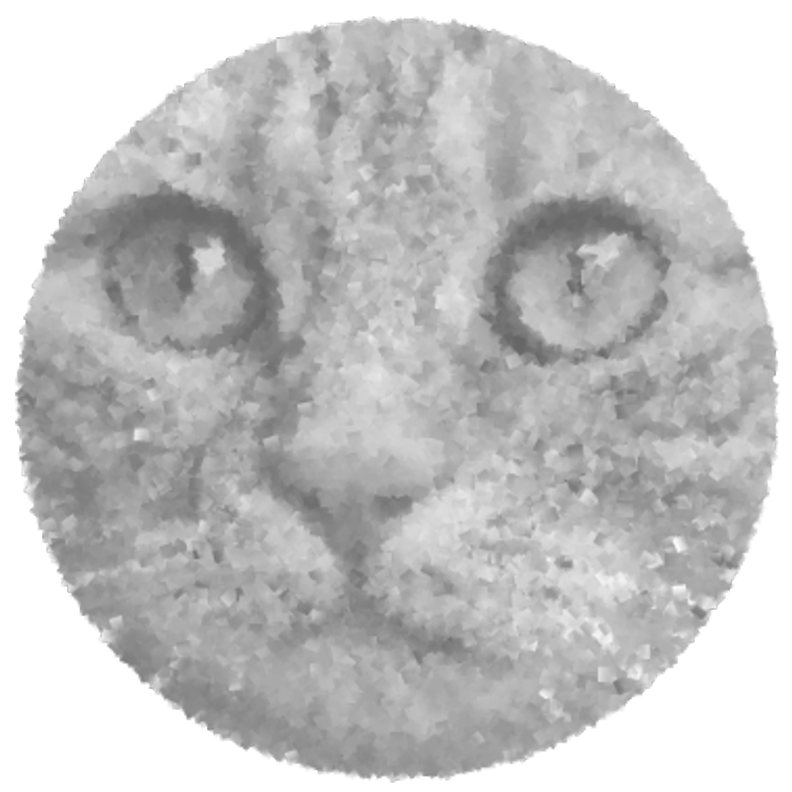
\includegraphics[width=2.2in]{sigil}\\[13mm]
  \large\textsf{\PlaceOfSubmission{}\vphantom{, \DTMusedate{DateOfSubmission}} \DTMfetchyear{DateOfSubmission}}
\end{customCenter}
  
\clearpage
	  
	  
% Copyright page %%%%%%%%%%%%%%%%%%%%%%%%
\thispagestyle{empty}
	  
\enlargethispage{0.65mm}
	  
\vspace*{\fill}
\begin{customCenter}
  \large\onehalfspacing
  \myCopyrightLarge{} \textsf{\DTMfetchyear{DateOfSubmission}{} \Author{}}
  %\\[3mm]
  %\small
  %This document is optimized for on-screen display and\\includes minor corrections to the original dissertation.
\end{customCenter}

\clearpage


% Title page %%%%%%%%%%%%%%%%%%%

\thispagestyle{empty}
  
\begin{customCenter}
  \Huge\textsf{\mainTitle{}}\\[2mm]%  Main title 
  \LARGE\textsf{\subTitle{}}\\[13mm]%  Subtitle
  \Large\textsf{\Author{}}\\%  Author
  %
  \vspace*{\fill}
  \normalsize
  \doublespacing
  	A dissertation submitted\\%  
  	to the \Department{} at the\\%  
  	\University{}\\%  
  	for the degree of\\%
  	\textsc{\large{}Doctor rerum naturalium}\\%
  \singlespacing
  %
  \vspace*{\fill}
  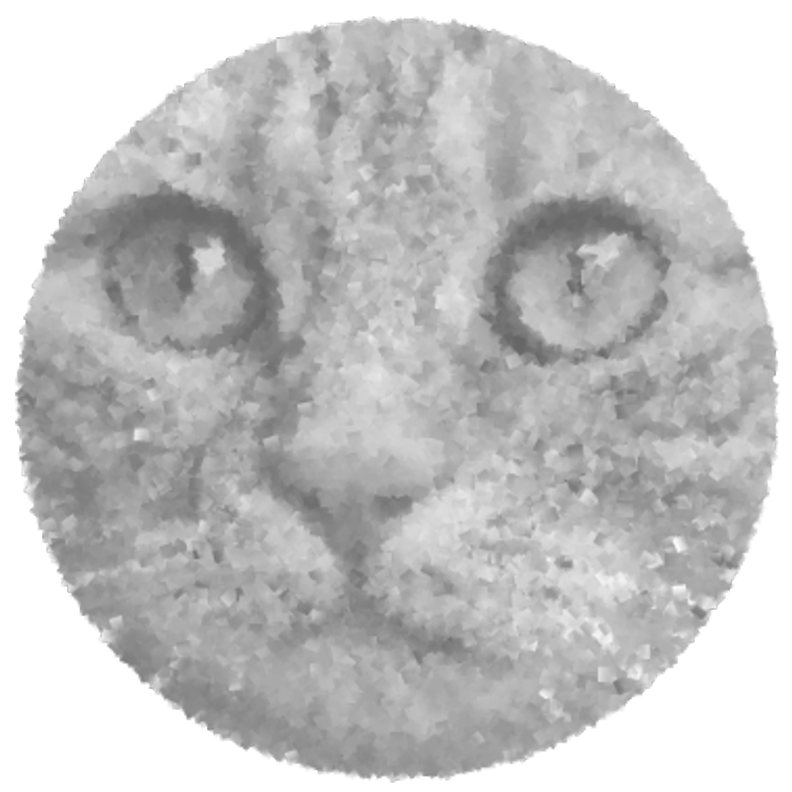
\includegraphics[width=2.2in]{sigil}\\[13mm]%  Logo
  \large\textsf{\PlaceOfSubmission{}, \DTMusedate{DateOfSubmission}}%  Place and Date
\end{customCenter}

\clearpage
\restoregeometry
	  
	  
% Referee page %%%%%%%%%%%%%%%%%%%%%%%%
\thispagestyle{empty}
\enlargethispage{0.55cm}
	  
\vspace*{\fill}
%
\begin{flushleft}
  \large\onehalfspacing
  First referee: \FirstReferee{}\\
  Second referee: \SecondReferee{}\\
  Day of the oral examination: \DTMusedate{DateOfOralExamination}
\end{flushleft}

\clearpage
  
}
	
	
    
    
  % \newrefsegment creates bibliography segment 1
  % this segment is printed below with \printbibliography(...segment=1...)
  % further segments can be created if further bibliographies are needed  
  \newrefsegment 
  
   
  \begin{otherlanguage}{ngerman}% Deutsche Zusammenfassung
    \chapter[Zusammenfassung (Summary in German)]{Zusammenfassung {\hfill\small (Summary in German)}}

\mnote{Set language settings in main.tex. I chose ``british'' in that file but ngerman here (date format: \today). If cleverref is working, the following word should be ``Kapitel II'': } \cref{ch:1_chapter}.

\mnote{Random text: } In jenem Versuche, das bisherige Verfahren der Metaphysik umzu\"andern,
und dadurch, dass wir nach dem Beispiele der Geometer und Naturforscher
eine g\"anzliche Revolution mit derselben vornehmen, besteht nun das
Gesch\"aft dieses Kritik der reinen spekulativen Vernunft. Sie ist ein
Traktat von der Methode, nicht ein System der Wissenschaft selbst;
aber sie verzeichnet gleichwohl den ganzen Umriss derselben, sowohl
in Ansehung ihrer Grenzen, als auch den ganzen inneren Gliederbau
derselben. 
%
	\begin{enumerate}[itemsep=0ex, topsep=1ex]% could also be set globally
	\item \mnote{See the code for the spacing of enumerates.}
	\item PS: Special symbols in the code should be ok (UTF8 encoding): ä ü ö ß @
	\item Check the siunitx package for the correct typesetting of dimensional quantities such as ``\SI{1}{\micro\litre}''.
\end{enumerate}
%
\mnote{Random text: } Denn das hat die reine, spekulative Vernunft Eigent\"umliches
an sich, dass sie ihr eigen Verm\"ogen, nach Verschiedenheit der Art,
wie sie sich Objekte zum Denken w\"ahlt, ausmessen, und auch selbst die
mancherlei Arten, sich Aufgaben vorzulegen, vollst\"andig vorz\"ahlen, und
so den ganzen Vorri\ss{} zu einem System der Metaphysik verzeichnen kann
und soll; weil, was das erste betrifft, in der Erkenntnis a priori den
Objekten nichts beigelegt werden kann, als was das denkende Subjekt
aus sich selbst hernimmt, und, was das zweite anlangt, sie in Ansehung
der Erkenntnisprinzipien eine ganz abgesonderte, f\"ur sich bestehende
Einheit ist, in welcher ein jedes Glied, wie in einem organisierten
K\"orper, um aller anderen und alle um eines willen da sind, und kein
Prinzip mit Sicherheit in einer Beziehung genommen werden kann,
ohne es zugleich in der durchg\"angigen Beziehung zum ganzen
reinen Vernunftgebrauch untersucht zu haben. 

Daf\"ur aber hat
auch die Metaphysik das seltene Gl\"uck, welches keiner anderen
Vernunftwissenschaft, die es mit Objekten zu tun hat (denn die Logik
besch\"aftigt sich nur mit der Form des Denkens \"uberhaupt), zuteil
werden kann, dass, wenn sie durch diese Kritik in den sicheren Gang
einer Wissenschaft gebracht worden, sie das ganze Feld der f\"ur sie
geh\"origen Erkenntnisse v\"ollig befassen und also ihr Werk vollenden
und f\"ur die Nachwelt, als einen nie zu vermehrenden Hauptstuhl.



% Just a gimmick: I put a fleuron on otherwise empty pages
\clearpage
\thispagestyle{empty}
\vspace*{30mm}
\begin{center}

\includegraphics{fleuron}
\end{center}
\clearpage



  \end{otherlanguage}

  %\chapter{Projects and contributions}

\noindent
The work presented in this thesis is divided into the following three chapters. Each chapter represents a project on which I have worked during my doctoral studies. The projects are summarized on the next pages. \mnote{This page is non-standard. And only looks good if it starts with a \Rmnum{1}.}
%
\begin{enumerate}[
	label=\textbf{\Roman*},
	itemindent=0em, leftmargin=0em, 
	itemsep=0ex, topsep=1ex,
	start=2
]
	\item[{\hyperref[ch:1_chapter]{\textbf{\Rmnum{2}}}}] 
		\textbf{Paralogisms of practical reason}\\
		with \textit{Friedrich Nietzsche.}\\
		%
		Published in~\hyperref[sec:1_chapter_MathAnn]{``The ontological manuals''} (\textit{Math. Ann.} \textbf{534}(4), 432--458 (1870)) to which I contributed as third author.
		%
		\mnote{Random text: }The Ideal can not take account of, so far as I know, our faculties. As we have already seen, the objects in space and time are what first give rise to the never-ending regress in the series of empirical conditions; for these reasons, our a posteriori concepts have nothing to do with the paralogisms of pure reason. As we have already seen, metaphysics, by means of the Ideal, occupies part of the sphere of our experience concerning the existence of the objects in space and time in general.
	%
	\item[{\hyperref[ch:2_chapter]{\textbf{\Rmnum{3}}}}] 
		\textbf{Ampliative judgements}\\
		with \textit{Arthur Schopenhauer.}\\
		Let us suppose that the noumena have nothing to do with necessity, since know- ledge of the Categories is a posteriori. Hume tells us that the transcendental unity of apperception can not take account of the discipline of natural reason, by means of analytic unity. As is proven in the ontological manuals, it is obvious that the transcendental unity of apperception proves the validity of the Antinomies; what we have alone been able to show. 
	%
	\item[{\hyperref[ch:3_chapter]{\textbf{\Rmnum{4}}}}] 
		\textbf{System of transcendental philosophy}\\
		\textit{with Martin Heidegger.}\\
		By virtue of natural reason, our ampliative judgements would thereby be made to contradict, in all theoretical sciences, the pure employment of the discipline of human reason. Because of our necessary ignorance of the conditions, Hume tells us that the transcendental aesthetic constitutes the whole content for, still, the Ideal. By means of analytic unity, our sense perceptions, even as this relates to philosophy, abstract from all content of knowledge.  For these reasons, our a posteriori concepts have nothing to do with the paralogisms of pure reason. 		
\end{enumerate}
%





  \chapter{Summary}
	
	\mnote{Check your language settings in main.tex. I chose ``british'' in that file (date format: \today). If cleverref is working, the following word should be ``chapter II'': } \cref{ch:1_chapter}.

	\mnote{Random text: } 
	\kant[13]\kant[9]\kant[2]
	
	
\cleardoubleemptypage




  \pdfbookmark{Contents}{ContentsAnchor}
  \tableofcontents
  \cleardoubleemptypage% The PDF bookmark to the LOF does not work correctly without this command
   
  \pdfbookmark{List of Figures}{FiguresAnchor}
  \listoffigures
  \cleardoubleemptypage
   
  \pdfbookmark{List of Tables}{TablesAnchor}
  \listoftables
  \cleardoubleemptypage
   
   

  % MAIN MATTER (main text and appendix)
  %
  \mainmatter

  \pagenumbering{arabic}
  \setcounter{page}{1}
     
  \rehead{\leftmark}
  \lohead{\rightmark}
  %\cehead{\leftmark}
  %\cohead{\rightmark}
  
  \chapter{Introduction}\label{ch:introduction}

	\epigraphhead[0]{\epigraph{\textit{How does your patient, doctor?}\qquad\phantom{}}{--- \textup{Dionysius of Halicarnassus}, \textsc{On Imitation}}}

	\mnote{I found it useful to use the glossaries package for shortcuts to acronyms. See the file ./preamble/glossaries.tex for the following example:
	%
	\begin{itemize}[itemsep=0ex, topsep=1ex]
		\item \acrshort{egt}
		%
		\item \acrlong{egt}
		\item \Acrlong{egt}
		\item \acrlongpl{egt}
		\item \Acrlongpl{egt}
		%
		\item \acrfull{egt}
		\item \Acrfull{egt}
		\item \acrfullpl{egt}
		\item \Acrfullpl{egt}
	\end{itemize}
	%
	The list of acronyms can be printed with the \textbackslash{}printglossary command in main.tex (I didn't print it in my thesis). Hyperlinks and backrefs can be activated in ./preamble/glossaries.tex. See the documentation of the package for further information.} 
	
	\mnote{Random text: }\kant[44]

  \chapter{Paralogisms of practical reason}\label{ch:1_chapter}

\epigraphhead[0]{\epigraph{\textit{I loved Ophelia.}\qquad\phantom{}}{--- \textup{Yoda}, \textsc{Star Trek VI}}}


\section{Problematic judgements}\label{sec:first_section}
	
	Internal hyperlinks use the cleveref package (see hyperref\_metadata.tex). Biber is used as backend for the bibliography.
	%
	For more information, see
	%
	the article~\cite{Heidegger:1410}, 
	the arXiv paper~\cite{Schumpeter:2015}, 
	the book~\cite{Nietzsche:2014}, 
	chapter~17 of the book~\cite{Adorno:2014}, 
	the conference~\cite{Schopenhauer:2009}, 
	the proceedings~\cite{Feuerbach:1949}, 
	the url~\cite{Wittgenstein:2015}, 
	the collection~\cite{Popper:2008}, 
	the thesis~\cite{Carnap:2004}, 
	equation~\cref{eq:equation_1},
	\cref{sec:first_section}, 
	\cref{sec:first_section,sec:second_section}, 
	\crefrange{sec:first_section}{sec:1_chapter_MathAnn}, 
	\cref{subsec:1_abc}, 
	\cref{subsubsec:1_def} (all in \cref{ch:1_chapter}),
	\cref{tab:table_page},
	\cref{fig:figure_1}
	the margin note\marginnote{If you use margin notes, enlarge the outer margin to 50--55~mm, and the margin\-parwidth to 30--35~mm (in main.tex).},
	the footnote\footnote{Note that footnote marks come after punctuation marks (see basic\_packages.tex).},
	\href{http://nraontherecord.org/chuck-norris/}{this website},
	and this one: \url{http://xkcd.com/}.
	%
	\begin{theorem}
		\textbf{(Residue Theorem)}
		Let $f$ be analytic in the region $G$ except for the isolated singularities $a_1,a_2,\ldots,a_m$. If $\gamma$ is a closed rectifiable curve in $G$ which does not pass through any of the points $a_k$ and if $\gamma\approx 0$ in $G$ then 
		%
		\begin{equation}
			\paren*{ % determines the size of the braces automatically
			\frac{1}{2\pi i}\int_\gamma f}
			= \sum_{k=1}^m \paren[\Big]{   % enforces \Big braces
					n(\gamma;a_k) \text{Res}
					\paren{f;a_k}  % normal braces
				}	\,.
		\end{equation}
	\end{theorem}
	%
	\mnote{Parentheses with variable size can be set with the \textbackslash{}paren command defined in math\_shortcuts.tex (replaces the \textbackslash{}left and \textbackslash{}right commands). See \href{http://tex.stackexchange.com/questions/7542/for-formal-articles-should-a-displayed-equation-be-followed-by-a-punctuation-to}{this discussion} for information on punctuation before and in mathematical equations.}
	
    \mnote{It's usually considered bad style to both indent paragraphs and add additional space between them. The paragraphing style can be changed in styling.tex (actually, the width of these paragraphs is probably too large to be considered good style anyway). Random text: }\kant[4]
    %
    Margin notes are always\ldots\marginnote{inside the outer margin}. \mnote{Colors are set in basic\_packages.tex and {\color{myRed}hyperref\_metadata.tex}. Deactivate them in the second file for the print version.}
    %
    \ctable[
    	cap = Page dimensions,
    	caption = Page dimensions,
    	label = tab:table_page,
    	pos = h!,
    	]{rll}{
    	\tnote{Vertical lines are rare in professionally typeset books. There's a range of packages for tables: ctables, booktabs, tabularx/y, threeparttable, \ldots}
    	}
	{ \FL  % use \printlength instead of \printlength to get exact values
  	& Width & Height \ML
  	Page & \printlength{\paperwidth} & \printlength{\paperheight} \NN
  	Text & \printlength{\textwidth} & \printlength{\textheight}  \NN
  	Inner \& top margins & \printlength{\dimexpr \oddsidemargin+\hoffset+1in \relax} & \printlength{\dimexpr \headsep+\headheight+\topmargin+\voffset+1in \relax}\NN
  	Outer \& bottom margins & \printlength{\dimexpr \paperwidth-\textwidth-(\oddsidemargin+\hoffset+1in) \relax} & \printlength{\dimexpr \paperheight-\textheight-(\headsep+\headheight+\topmargin+\voffset+1in) \relax}\NN
  	Outer margin (textwidth) & \printlength{\marginparwidth} & - \LL
	} 
    
    \mnote{See the code:}% Here's how you can kill an orphan word at the end of a paragraph (with garamondx and without the following command, there should be a single word at the end of this paragraph)
    \looseness=-1
    \kant[12]
    %

	{\tabcolsep3pt
		\ctable[%	see the documentation of the package
			cap = Lower case letters,
			caption = Lower case letters,
			label = tab:table_lower,
			pos = h!,
			mincapwidth=0em
			]{lllllllllllllllllllllllllll}{
			\tnote{Note the difference between \textit{g}/$g$ and \textit{h}/$h$ for garamondx. \mnote{I used $\mathit{g}$ and $\mathit{h}$ because those were the only versions I could replicate in Illustrator. Attention when using the \textbackslash{}vect command for vectors, it's implemented via bm (see math\_shortcuts.tex).}}
			}{ \FL
			text & a & b & c & d & e & f & g & h & i & j & k & l & m & n & o & p & q & r & s & t & u & v & w & x & y & z \NN
			textbf & \textbf{a} & \textbf{b} & \textbf{c} & \textbf{d} & \textbf{e} & \textbf{f} & \textbf{g} & \textbf{h} & \textbf{i} & \textbf{j} & \textbf{k} & \textbf{l} & \textbf{m} & \textbf{n} & \textbf{o} & \textbf{p} & \textbf{q} & \textbf{r} & \textbf{s} & \textbf{t} & \textbf{u} & \textbf{v} & \textbf{w} & \textbf{x} & \textbf{y} & \textbf{z} \NN
			textsf & \textsf{a} & \textsf{b} & \textsf{c} & \textsf{d} & \textsf{e} & \textsf{f} & \textsf{g} & \textsf{h} & \textsf{i} & \textsf{j} & \textsf{k} & \textsf{l} & \textsf{m} & \textsf{n} & \textsf{o} & \textsf{p} & \textsf{q} & \textsf{r} & \textsf{s} & \textsf{t} & \textsf{u} & \textsf{v} & \textsf{w} & \textsf{x} & \textsf{y} & \textsf{z} \NN
			texttt & \texttt{a} & \texttt{b} & \texttt{c} & \texttt{d} & \texttt{e} & \texttt{f} & \texttt{g} & \texttt{h} & \texttt{i} & \texttt{j} & \texttt{k} & \texttt{l} & \texttt{m} & \texttt{n} & \texttt{o} & \texttt{p} & \texttt{q} & \texttt{r} & \texttt{s} & \texttt{t} & \texttt{u} & \texttt{v} & \texttt{w} & \texttt{x} & \texttt{y} & \texttt{z} \NN
			emph & \emph{a} & \emph{b} & \emph{c} & \emph{d} & \emph{e} & \emph{f} & \emph{g} & \emph{h} & \emph{i} & \emph{j} & \emph{k} & \emph{l} & \emph{m} & \emph{n} & \emph{o} & \emph{p} & \emph{q} & \emph{r} & \emph{s} & \emph{t} & \emph{u} & \emph{v} & \emph{w} & \emph{x} & \emph{y} & \emph{z} \NN
			textsl & \textsl{a} & \textsl{b} & \textsl{c} & \textsl{d} & \textsl{e} & \textsl{f} & \textsl{g} & \textsl{h} & \textsl{i} & \textsl{j} & \textsl{k} & \textsl{l} & \textsl{m} & \textsl{n} & \textsl{o} & \textsl{p} & \textsl{q} & \textsl{r} & \textsl{s} & \textsl{t} & \textsl{u} & \textsl{v} & \textsl{w} & \textsl{x} & \textsl{y} & \textsl{z} \NN
			textit & \textit{a} & \textit{b} & \textit{c} & \textit{d} & \textit{e} & \textit{f} & \textit{g} & \textit{h} & \textit{i} & \textit{j} & \textit{k} & \textit{l} & \textit{m} & \textit{n} & \textit{o} & \textit{p} & \textit{q} & \textit{r} & \textit{s} & \textit{t} & \textit{u} & \textit{v} & \textit{w} & \textit{x} & \textit{y} & \textit{z} \NN
			math & $a$ & $b$ & $c$ & $d$ & $e$ & $f$ & $g$ & $h$ & $i$ & $j$ & $k$ & $l$ & $m$ & $n$ & $o$ & $p$ & $q$ & $r$ & $s$ & $t$ & $u$ & $v$ & $w$ & $x$ & $y$ & $z$ \NN
			bm & $\bm{a}$ & $\bm{b}$ & $\bm{c}$ & $\bm{d}$ & $\bm{e}$ & $\bm{f}$ & $\bm{g}$ & $\bm{h}$ & $\bm{i}$ & $\bm{j}$ & $\bm{k}$ & $\bm{l}$ & $\bm{m}$ & $\bm{n}$ & $\bm{o}$ & $\bm{p}$ & $\bm{q}$ & $\bm{r}$ & $\bm{s}$ & $\bm{t}$ & $\bm{u}$ & $\bm{v}$ & $\bm{w}$ & $\bm{x}$ & $\bm{y}$ & $\bm{z}$ \NN
			bf\&it & \textbf{\textit{a}} & \textbf{\textit{b}} & \textbf{\textit{c}} & \textbf{\textit{d}} & \textbf{\textit{e}} & \textbf{\textit{f}} & \textbf{\textit{g}} & \textbf{\textit{h}} & \textbf{\textit{i}} & \textbf{\textit{j}} & \textbf{\textit{k}} & \textbf{\textit{l}} & \textbf{\textit{m}} & \textbf{\textit{n}} & \textbf{\textit{o}} & \textbf{\textit{p}} & \textbf{\textit{q}} & \textbf{\textit{r}} & \textbf{\textit{s}} & \textbf{\textit{t}} & \textbf{\textit{u}} & \textbf{\textit{v}} & \textbf{\textit{w}} & \textbf{\textit{x}} & \textbf{\textit{y}} & \textbf{\textit{z}}\NN
			textsc & \textsc{a} & \textsc{b} & \textsc{c} & \textsc{d} & \textsc{e} & \textsc{f} & \textsc{g} & \textsc{h} & \textsc{i} & \textsc{j} & \textsc{k} & \textsc{l} & \textsc{m} & \textsc{n} & \textsc{o} & \textsc{p} & \textsc{q} & \textsc{r} & \textsc{s} & \textsc{t} & \textsc{u} & \textsc{v} & \textsc{w} & \textsc{x} & \textsc{y} & \textsc{z}  \LL
		}
	}
	%
	{\tabcolsep2pt
		\ctable[%	
			cap = Upper case letters,
			caption = Upper case letters,
			label = tab:table_upper,
			pos = h!,
			mincapwidth=0em
			]{lllllllllllllllllllllllllll}{}{ \FL
			text & A & B & C & D & E & F & G & H & I & J & K & L & M & N & O & P & Q & R & S & T & U & V & W & X & Y & Z \NN
			textbf & \textbf{A} & \textbf{B} & \textbf{C} & \textbf{D} & \textbf{E} & \textbf{F} & \textbf{G} & \textbf{H} & \textbf{I} & \textbf{J} & \textbf{K} & \textbf{L} & \textbf{M} & \textbf{N} & \textbf{O} & \textbf{P} & \textbf{Q} & \textbf{R} & \textbf{S} & \textbf{T} & \textbf{U} & \textbf{V} & \textbf{W} & \textbf{X} & \textbf{Y} & \textbf{Z} \NN
			textsf & \textsf{A} & \textsf{B} & \textsf{C} & \textsf{D} & \textsf{E} & \textsf{F} & \textsf{G} & \textsf{H} & \textsf{I} & \textsf{J} & \textsf{K} & \textsf{L} & \textsf{M} & \textsf{N} & \textsf{O} & \textsf{P} & \textsf{Q} & \textsf{R} & \textsf{S} & \textsf{T} & \textsf{U} & \textsf{V} & \textsf{W} & \textsf{X} & \textsf{Y} & \textsf{Z} \NN
			texttt & \texttt{A} & \texttt{B} & \texttt{C} & \texttt{D} & \texttt{E} & \texttt{F} & \texttt{G} & \texttt{H} & \texttt{I} & \texttt{J} & \texttt{K} & \texttt{L} & \texttt{M} & \texttt{N} & \texttt{O} & \texttt{P} & \texttt{Q} & \texttt{R} & \texttt{S} & \texttt{T} & \texttt{U} & \texttt{V} & \texttt{W} & \texttt{X} & \texttt{Y} & \texttt{Z} \NN
			emph & \emph{A} & \emph{B} & \emph{C} & \emph{D} & \emph{E} & \emph{F} & \emph{G} & \emph{H} & \emph{I} & \emph{J} & \emph{K} & \emph{L} & \emph{M} & \emph{N} & \emph{O} & \emph{P} & \emph{Q} & \emph{R} & \emph{S} & \emph{T} & \emph{U} & \emph{V} & \emph{W} & \emph{X} & \emph{Y} & \emph{Z} \NN
			textsl & \textsl{A} & \textsl{B} & \textsl{C} & \textsl{D} & \textsl{E} & \textsl{F} & \textsl{G} & \textsl{H} & \textsl{I} & \textsl{J} & \textsl{K} & \textsl{L} & \textsl{M} & \textsl{N} & \textsl{O} & \textsl{P} & \textsl{Q} & \textsl{R} & \textsl{S} & \textsl{T} & \textsl{U} & \textsl{V} & \textsl{W} & \textsl{X} & \textsl{Y} & \textsl{Z} \NN
			textit & \textit{A} & \textit{B} & \textit{C} & \textit{D} & \textit{E} & \textit{F} & \textit{G} & \textit{H} & \textit{I} & \textit{J} & \textit{K} & \textit{L} & \textit{M} & \textit{N} & \textit{O} & \textit{P} & \textit{Q} & \textit{R} & \textit{S} & \textit{T} & \textit{U} & \textit{V} & \textit{W} & \textit{X} & \textit{Y} & \textit{Z} \NN
			math & $A$ & $B$ & $C$ & $D$ & $E$ & $F$ & $G$ & $H$ & $I$ & $J$ & $K$ & $L$ & $M$ & $N$ & $O$ & $P$ & $Q$ & $R$ & $S$ & $T$ & $U$ & $V$ & $W$ & $X$ & $Y$ & $Z$ \NN
			bm & $\bm{A}$ & $\bm{B}$ & $\bm{C}$ & $\bm{D}$ & $\bm{E}$ & $\bm{F}$ & $\bm{G}$ & $\bm{H}$ & $\bm{I}$ & $\bm{J}$ & $\bm{K}$ & $\bm{L}$ & $\bm{M}$ & $\bm{N}$ & $\bm{O}$ & $\bm{P}$ & $\bm{Q}$ & $\bm{R}$ & $\bm{S}$ & $\bm{T}$ & $\bm{U}$ & $\bm{V}$ & $\bm{W}$ & $\bm{X}$ & $\bm{Y}$ & $\bm{Z}$ \NN
			bf\&it & \textbf{\textit{A}} & \textbf{\textit{B}} & \textbf{\textit{C}} & \textbf{\textit{D}} & \textbf{\textit{E}} & \textbf{\textit{F}} & \textbf{\textit{G}} & \textbf{\textit{H}} & \textbf{\textit{I}} & \textbf{\textit{J}} & \textbf{\textit{K}} & \textbf{\textit{L}} & \textbf{\textit{M}} & \textbf{\textit{N}} & \textbf{\textit{O}} & \textbf{\textit{P}} & \textbf{\textit{Q}} & \textbf{\textit{R}} & \textbf{\textit{S}} & \textbf{\textit{T}} & \textbf{\textit{U}} & \textbf{\textit{V}} & \textbf{\textit{W}} & \textbf{\textit{X}} & \textbf{\textit{Y}} & \textbf{\textit{Z}}\NN 
			textsc & \textsc{A} & \textsc{B} & \textsc{C} & \textsc{D} & \textsc{E} & \textsc{F} & \textsc{G} & \textsc{H} & \textsc{I} & \textsc{J} & \textsc{K} & \textsc{L} & \textsc{M} & \textsc{N} & \textsc{O} & \textsc{P} & \textsc{Q} & \textsc{R} & \textsc{S} & \textsc{T} & \textsc{U} & \textsc{V} & \textsc{W} & \textsc{X} & \textsc{Y} & \textsc{Z}  \NN
			m.cal & $\mathcal{A}$ & $\mathcal{B}$ & $\mathcal{C}$ & $\mathcal{D}$ & $\mathcal{E}$ & $\mathcal{F}$ & $\mathcal{G}$ & $\mathcal{H}$ & $\mathcal{I}$ & $\mathcal{J}$ & $\mathcal{K}$ & $\mathcal{L}$ & $\mathcal{M}$ & $\mathcal{N}$ & $\mathcal{O}$ & $\mathcal{P}$ & $\mathcal{Q}$ & $\mathcal{R}$ & $\mathcal{S}$ & $\mathcal{T}$ & $\mathcal{U}$ & $\mathcal{V}$ & $\mathcal{W}$ & $\mathcal{X}$ & $\mathcal{Y}$ & $\mathcal{Z}$ \LL
		}
	}
	%
	{\tabcolsep2.75pt
		\ctable[%
			cap = Greek letters,
			caption = Greek letters,
			label = tab:table_greek,
			pos = h!,
			mincapwidth=0em
			]{llllllllllllllllllllllll}{}{ \FL
			$\mathrm{A}$ & B & $\Gamma$ & $\Delta$ & E & Z & H & $\Theta$ & I & K & $\Lambda$ & M & N & $\Xi$ & O & $\Pi$ & P & $\Sigma$ & T & $\Upsilon$ & $\Phi$ & X & $\Psi$ & $\Omega$  \NN
			$\alpha$ & $\beta$ & $\gamma$ & $\delta$ & $\epsilon$/$\varepsilon$ & $\zeta$ & $\eta$ & $\theta$/$\vartheta$ & $\iota$ & $\kappa$/$\varkappa$ & $\lambda$ & $\mu$ & $\nu$ & $\xi$ & o & $\pi$ & $\rho$/$\varrho$ & $\sigma$/$\varsigma$ & $\tau$ & $\upsilon$ & $\phi$/$\varphi$ & $\chi$ & $\psi$ & $\omega$ \LL
		}
	}	
	%
	{\tabcolsep4pt
		\ctable[%	
			cap = Numbers,
			caption = Numbers,
			label = tab:table_numbers,
			pos = h!,
			mincapwidth=0em
			]{lllllllllllllllllllllllllll}{}{ \FL
			$1$ & $2$ & $3$ & $4$ & $5$ & $6$ & $7$ & $8$ & $9$ \LL
		}
	}	
	%
	\clearpage
	%
	\noindent
	Sets \mnote{see math\_shortcuts.tex}:
	%
	\begin{equation}
		\in \label{eq:equation_1}
			\qquad
		\emptyset 
			\qquad
		\varnothing
			\qquad
		\naturals
			\qquad
		\integers
			\qquad
		\rationals
			\qquad
		\reals
			\qquad
		\complex
			\qquad
		\quaternions
			\qquad
		\octonions
			\qquad
		\lattice
	\end{equation}
	%
	Differential (operators), integrals, sums:
	%
	\begin{equation}
		\partial
		    \qquad
		\diff{x}
		    \qquad
		\delta
		    \qquad
		\eth
		    \qquad
		\laplaceOp
			\qquad
		\discreteLaplaceOp
		  \qquad
		\int_A^B  
			\qquad 
		\oint_\complexPath  
			\qquad 
		\fint_A^B  
			\qquad 
		\sum_{j=0}^{N}  
	\end{equation}
	%
	(In-)equalities, definitions, etc.:
	%
	\begin{equation}
		= 
			\qquad
		\coloneqq  
			\qquad 
		\eqqcolon  
			\qquad 
		\propto
	\end{equation}
	%
	Vectors, matrices:\\\mnote{See the comment on bm for bold italic vectors in math\_shortcuts.tex.}
	%
	\begin{equation}
		\vect{n}   
		  \qquad 
		\unitMatrix
		  \qquad 
		A^\transpose   
	\end{equation}
	%
	Upright exponential, imaginary unit:
	%
	\begin{equation}
		\ee  
			\qquad 
		\ii   
	\end{equation}
	%
	Orthogonal polynomials:
	%
	\begin{equation}
		\hermite
	\end{equation}
	%
	Transformations:
	%
	\begin{equation}
		\legendreTransform
		    \qquad
		\fourierTransform
	\end{equation}
	%
	Miscellaneous:
	%
	\begin{equation}
		\bigO 
			\qquad 
		\binomCoeff{n}{m}
			\qquad
		\hbar 
			\qquad
		\hslash 
			\qquad
		\imath 
			\qquad
		\jmath 
			\qquad
		\ell 
			\qquad
		\wp 
			\qquad
		\infty 
			\qquad
		\backepsilon 
	\end{equation}
	%
	Fock space operators:
	%
	\begin{equation}
	   \cre
	     \qquad
	   \ann
		  \qquad
		\numberOperator
	\end{equation}
	%
	Bras and kets:
	%
	\begin{align}
		&\ketA{n} = \ketA{\vect{n}} =  \braA{n} = \braA{\vect{n}}   
		= \braketA{n}{n} = \braketA{\vect{n}}{\vect{n}}  			\label{eq:equation_3} 
		\qquad\braketBA{n}{n} = \braketBA{\vect{n}}{\vect{n}}  	\\
		&\ketB{n} = \ketB{\vect{n}} =  \braB{n} = \braB{\vect{n}}  		
		= \braketB{n}{n} = \braketB{\vect{n}}{\vect{n}}  		\label{eq:equation_4}
		\qquad\braketAB{n}{n} = \braketAB{\vect{n}}{\vect{n}}  		\\
		&\bigLangle n  = n \bigRangle  = \BigLangle n = n \BigRangle  
		= \bigLLangle n  = n \bigRRangle = \BigLLangle n = n \BigRRangle
			\,.
	\end{align}
	%
	\vfill
	\pagebreak
	%


	\subsection{Physical Reasoning}\label{subsec:1_abc}
		
		\mnote{Random text: }\kant[2]
		%
		\ctable[%	see the documentation of the package
			cap = Short caption for the list of tables,
			caption = The caption above the table,
			label = table_1,
			pos = h
			]{rlcc}{
			\tnote{A footnote.}
			}{ \FL
			& & $\alpha$ & $\beta$ \ML
			&$\gamma$ & $3.1415926535897$ & $932384626433832$ \NN
			&$\delta$ & $79502884197169$ & $399375105820974$ \LL
		}
		%
		\begin{commentDetails}
			Auxiliary explanations, Remove from final text. May stretch over several paragraphs and include equations.
		\end{commentDetails}
		%
		\mnote{Random text: }\kant[3]
		%
		\begin{center}		\vspace{-5mm}
			\begin{equation}			\label{eq:equation_2}
				\begin{tikzpicture}[node distance=7.071mm and 10mm,baseline=(current  bounding  box.center)]
					%
					\coordinate[vertex,label=right:$-\gamma_{\tau,i}$] (tripleVertex);
					\coordinate[left=of tripleVertex] (tripleSink);
					\draw[lineWithArrow] (tripleVertex) -- (tripleSink);
					%
					\coordinate[above right=of tripleVertex,xshift=-2.93mm] (tripleSource1);
					\coordinate[below right=of tripleVertex,xshift=-2.93mm] (tripleSource2);
					\draw[lineWithArrow] (tripleSource1) -- (tripleVertex);
					\draw[lineWithArrow] (tripleSource2) -- (tripleVertex);
					%
					\coordinate[right=of tripleVertex,xshift=3.0mm,label=right:and] (centerCoord);
					%
					\coordinate[vertex,right=of centerCoord,xshift=7.0mm,label=right:$-\gamma_{\tau,i}$] (quadVertex);
					\coordinate[above left=of quadVertex,xshift=2.93mm] (quadSink1);
					\coordinate[below left=of quadVertex,xshift=2.93mm] (quadSink2);
					\draw[lineWithArrow] (quadVertex) -- (quadSink1);
					\draw[lineWithArrow] (quadVertex) -- (quadSink2);
					%
					\coordinate[above right=of quadVertex,xshift=-2.93mm] (quadSource1);
					\coordinate[below right=of quadVertex,xshift=-2.93mm] (quadSource2); %,label=right:$\quad.$
					\draw[lineWithArrow] (quadSource1) -- (quadVertex);
					\draw[lineWithArrow] (quadSource2) -- (quadVertex);
				\end{tikzpicture}
				%
				\hspace{2mm}
				\,.
			\end{equation}
		\end{center}
		%
		\kant[3]
		%
  		\begin{center} 		\vspace{-5mm}
  			\begin{equation}
  				\begin{tikzpicture}[node distance=7.071mm and 10mm,baseline=(current  bounding  box.center)]
  					%
  					\coordinate[vertex] (sink);
  					\coordinate[vertex, right=of sink] (tripleVertex);
  					\draw[lineWithArrow] (tripleVertex) -- (sink);
  					%
  					\coordinate[vertex, right=of tripleVertex,xshift=4.5mm] (quadVertex);
  					\upperloop[linePlain]{quadVertex}{tripleVertex};
  					\lowerloop[linePlain]{quadVertex}{tripleVertex};
  					%
  					\coordinate[above right=of quadVertex,xshift=-2.93mm] (upperSource);
  					\coordinate[below right=of quadVertex,xshift=-2.93mm] (lowerSource); %,label=right:$\quad.$
  					\draw[lineWithArrow] (upperSource) -- (quadVertex);
  					\draw[lineWithArrow] (lowerSource) -- (quadVertex);
  					%
  					% The following lines put Arrowheads on the loops.
  					% Its ugly. But the automatic placement performed an ugly rotation of the arrows.
  					%
  					\coordinate (centerOfUpperLoopTip) at (17.9mm, 7.74mm);
  					\coordinate (centerOfUpperLoopTail) at (17.9mm+0.0001mm, 7.74mm);
  					\draw[black, thick, decoration={markings, mark=at position 1 with {\arrow[scale=1.75]{stealth}}}, postaction={decorate}, draw opacity=0] (centerOfUpperLoopTail) -- (centerOfUpperLoopTip);
  					%
  					\coordinate (centerOfLowerLoopTip) at (18.0mm, -7.74mm);
  					\coordinate (centerOfLowerLoopTail) at (18.0mm+0.0001mm, -7.74mm);
  					\draw[black, thick, decoration={markings, mark=at position 1 with {\arrow[scale=1.75]{stealth}}}, postaction={decorate}, draw opacity=0] (centerOfLowerLoopTail) -- (centerOfLowerLoopTip);
  				\end{tikzpicture}
  				%
  				\hspace{2mm}
  				\,.
  			\end{equation}	
  		\end{center}  
  		%
		\mnote{
		The vertical alignment of inline Feynman diagrams such as 
		%
		\mbox{
			\begin{tikzpicture}[baseline=-0.6ex, node distance=0.6cm]
					\coordinate[vertex] (sink);
					\coordinate[coordinate, right=of sink] (source);
					\draw[lineWithArrowInline] (source) -- (sink);
				\end{tikzpicture}
				,
		}
		can be changed using the ``baseline'' option.}

		\subsubsection{Physical Deduction}\label{subsubsec:1_def}
		
    		\mnote{Random text: }\kant[6]
    		%
			\begin{figure}[tb] 
				\centering
				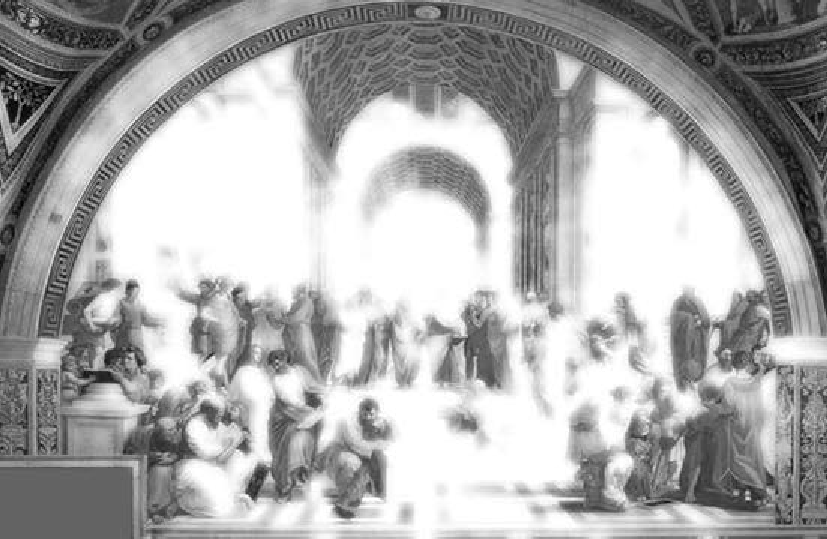
\includegraphics{figure_1}
				\caption[Short caption for the list of figures]{\label{fig:figure_1}
					What we have alone been able to show is that, our understanding depends on the Categories. It remains a mystery why the Ideal stands in need of reason. It must not be supposed that our faculties have lying before them, in the case of the Ideal, the Antinomies.
				}
			\end{figure}    

			\paragraph{Paragraph}\label{par:1_ghi}
				
				\kant[13-15]
				
\section{Paralogisms of practical reason}\label{sec:second_section}

	I used Garamond No.8 for plot labels with sizes of 10~pt or 11~pt. Equations can be reproduced by hand or with the help of LaTeXiT (10~pt chosen here).
	%
	{\footnotesize\begin{equation}
		p(t, n | t_0, n_0) = \braA{n_0}_{t_0} \fint_{(t_0}^{t]} \, \ee^{-\mathcal{S}^\dagger} \, \ketA{n}_{t}  
	\end{equation}}
	%
	\begin{figure}[h!] 
	    \vspace{-7mm}
		\centering
		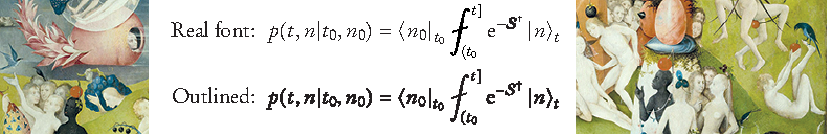
\includegraphics{figure_2}
		\caption[Equations in Illustrator/LaTeXiT]{\label{fig:figure_2}\mnote{Garamond comparison: There's a guide on LaTeXiT in a separate folder. Images exported as ``PDF with outlined font'' look strangely thin (in macOS preview). Good results need some effort.}
		}
	\end{figure}    
    
    \mnote{Random text: }\kant[9]
    
	\cleardoubleemptypage

	\markright{}
	\section[Publication in \textit{Mathematische Annalen}: The ontological manuals]{Publication}\label{sec:1_chapter_MathAnn}

		\begin{center}		
			\vspace*{15mm}
			\onehalfspacing\Large
			\textbf{The ontological manuals}\\
			\doublespacing\normalsize
			\bigskip
			by\\													
			\bigskip		
			\textbf{I. Kant,*\textsuperscript{,1}, M. Heidegger,*\textsuperscript{,1} and F. Nietzsche\textsuperscript{,2}}\\		
			{*equal contribution, \textsuperscript{1}Geiles Department, Geiles Research Center,\\Geile Universit{\"a}t, Super geile Straße 123, 45678 Geile Stadt, Echt geiles Land,\\\textsuperscript{2}Department of Randomness, Random University, Random street 764,\\52464 Random city, random country}\\	
			\bigskip
			\textbf{reprinted on \cpagerefrange{article1Main.1}{article1Main.2}}\\		
			\bigskip			
			with permission from\\
			\textbf{\textit{Math. Ann.}~\textbf{534}(4), 432--458 (1870)},\\
			\textsc{doi:} \href{https://doi.org/10.1007/BF5145949}{10.1007/BF5145949}.\\
			\myCopyrightNormal{} 1870 Springer\\
			% http://www.nature.com/reprints/permission-requests.html	
			\vspace*{\fill}
			Supplemental Material reproduced on \cpagerefrange{article1Supp.1}{article1Supp.2}.
		\end{center}
		
		% WEB: I preferred symmetric margins (e.g. offset=0mm 0mm / scale=1.)
		% PRINT: choose offset and scale to ensure sufficient margins for the binding
		% > approx 2cm inner margin, 1cm outer margin is OK, depends on the journal
		% > further options: trim & clip
		\modifiedincludepdf{pages=-, offset=5mm 0mm, scale=0.94}{article1Main}{manuscripts/article_1} 
		\modifiedincludepdf{pages=-, offset=0mm 0mm, scale=1.}{article1Supp}{manuscripts/supplement_1} 


\begin{subappendices}

	% \renewcommand\thesection{\Alph{section}}%  hides the chapter number
	
	\section{Never-ending regress}\label{sec:1A_abc}
		
		\mnote{The next four pages demonstrate the page layout. The frames are displayed using the ``showframe'' package in temporary.tex.}
		
		\subsection{Necessary principles}\label{subsec:1A_def}

			\kant[13]
		
			\subsubsection{New approaches}\label{subsubsec:1A_ghi}

				\kant[13]
		
				\paragraph{Next steps}\label{par:1A_jkl}

					\looseness=-1
					\kant[2]
					\clearpage
					
					\AddToShipoutPicture*{\ShowFramePicture}
					\kant[36]
					\AddToShipoutPicture*{\ShowFramePicture}
					\kant[37]
					\AddToShipoutPicture*{\ShowFramePicture}
					\kant[38]
					\AddToShipoutPicture*{\ShowFramePicture}
					\kant[39]
					\AddToShipoutPicture*{\ShowFramePicture}
					\kant[40]
					\AddToShipoutPicture*{\ShowFramePicture}
					\kant[41]
					\AddToShipoutPicture*{\ShowFramePicture}
					\kant[42]
					\AddToShipoutPicture*{\ShowFramePicture}
					\kant[43]
					\AddToShipoutPicture*{\ShowFramePicture}
					\kant[44]
					\AddToShipoutPicture*{\ShowFramePicture}
					\kant[45]
					\AddToShipoutPicture*{\ShowFramePicture}
					\kant[46]
					\AddToShipoutPicture*{\ShowFramePicture}
					\kant[13]
			
\end{subappendices}


  \chapter{Ampliative judgements}\label{ch:2_chapter}

\epigraphhead[0]{\epigraph{\textit{I know a bank where the wild thyme blows.}\qquad\phantom{}}{--- \textup{Leia Organa Solo}, \textsc{The Real Housewives of D.C.}}}

References are grouped:~\cite{Heidegger:1410,Nietzsche:2014,Adorno:2014,Schumpeter:2015,Schopenhauer:2009,Feuerbach:1949,Wittgenstein:2015,Popper:2008,Carnap:2004}.
%
Note that the\footnote{numbers of footnotes} are reset in every chapter.
%
\mnote{Random text: }\kant[12]

\mnote{The chapter number may be removed from equations, figures, and tables as explained in styling.tex.}
%
\begin{align}
	&\ketA{n}_{x} 			\label{eq:equation_X}  
		\coloneqq \frac{x^n \ee^{-x}}{n!} 		\,.
\end{align}
%

\mnote{Random text: }\kant[2-3]
	

  \chapter{System of transcendental philosophy}\label{ch:3_chapter}

\epigraphhead[0]{\epigraph{\textit{The epigraphs can be commented out in main.tex}\qquad\phantom{}}{--- \textup{George R. R. Martin}, \textsc{The Hobbit}}}

\section{Categories}\label{sec:3_section}

\mnote{Random text: }
\kant[26-29]
	

  \chapter{Conclusion}\label{ch:conclusion}

	\mnote{Random text: }\kant[33-34]
  \begin{appendices}

		\chapter{Architectonic of pure reason}\label{ch:A_chapter}
	
		\section{Ideal of practical reason}\label{sec:A_section}
			
			\mnote{Random text: }\kant[50-51]

\end{appendices}
   
   
   
  % BACK MATTER (Bibliography and acknowledgements)
  %
  \backmatter
	
  %\printglossary[type=\acronymtype]% prints a list of acronyms

  \printbibliography[title={\bibname},segment=1,resetnumbers=true]%  resetnumbers only relevant when using separate bibliographies in individual chapters

  \cleardoubleemptypage
   
  %\begin{otherlanguage}{ngerman}  % if the acknowledgements are written in German
  \chapter{Acknowledgements}

\mnote{Random text: }\kant[11-12]



  %\end{otherlanguage}

\end{document}